%======================================================================
\section{Experimental Protocol and Audit Trail}
\label{sec:protocol}
%======================================================================

\paragraph{Synchronous panels.}
Each question is processed by five agents for three synchronous rounds. In round $t$, an agent can observe only the permitted subset of round-$t-1$ reports; agents in the same round cannot observe one another. The confirmatory suite uses the independent information condition, so no peer content is visible. Controlled information suites later expose one new evidence item, only a majority stance, full peer reports with copy pressure, or stance-opposing evidence.

Figure~\ref{fig:runtime} makes the implemented ordering explicit. The controller commits first, each follower declares an action before solving, the executor runs the corresponding path, and only then does settlement create the history visible in subsequent rounds. Parse or API failures follow an auditable retry or rollback branch rather than silently changing the protocol.

\begin{figure}[t]
\centering
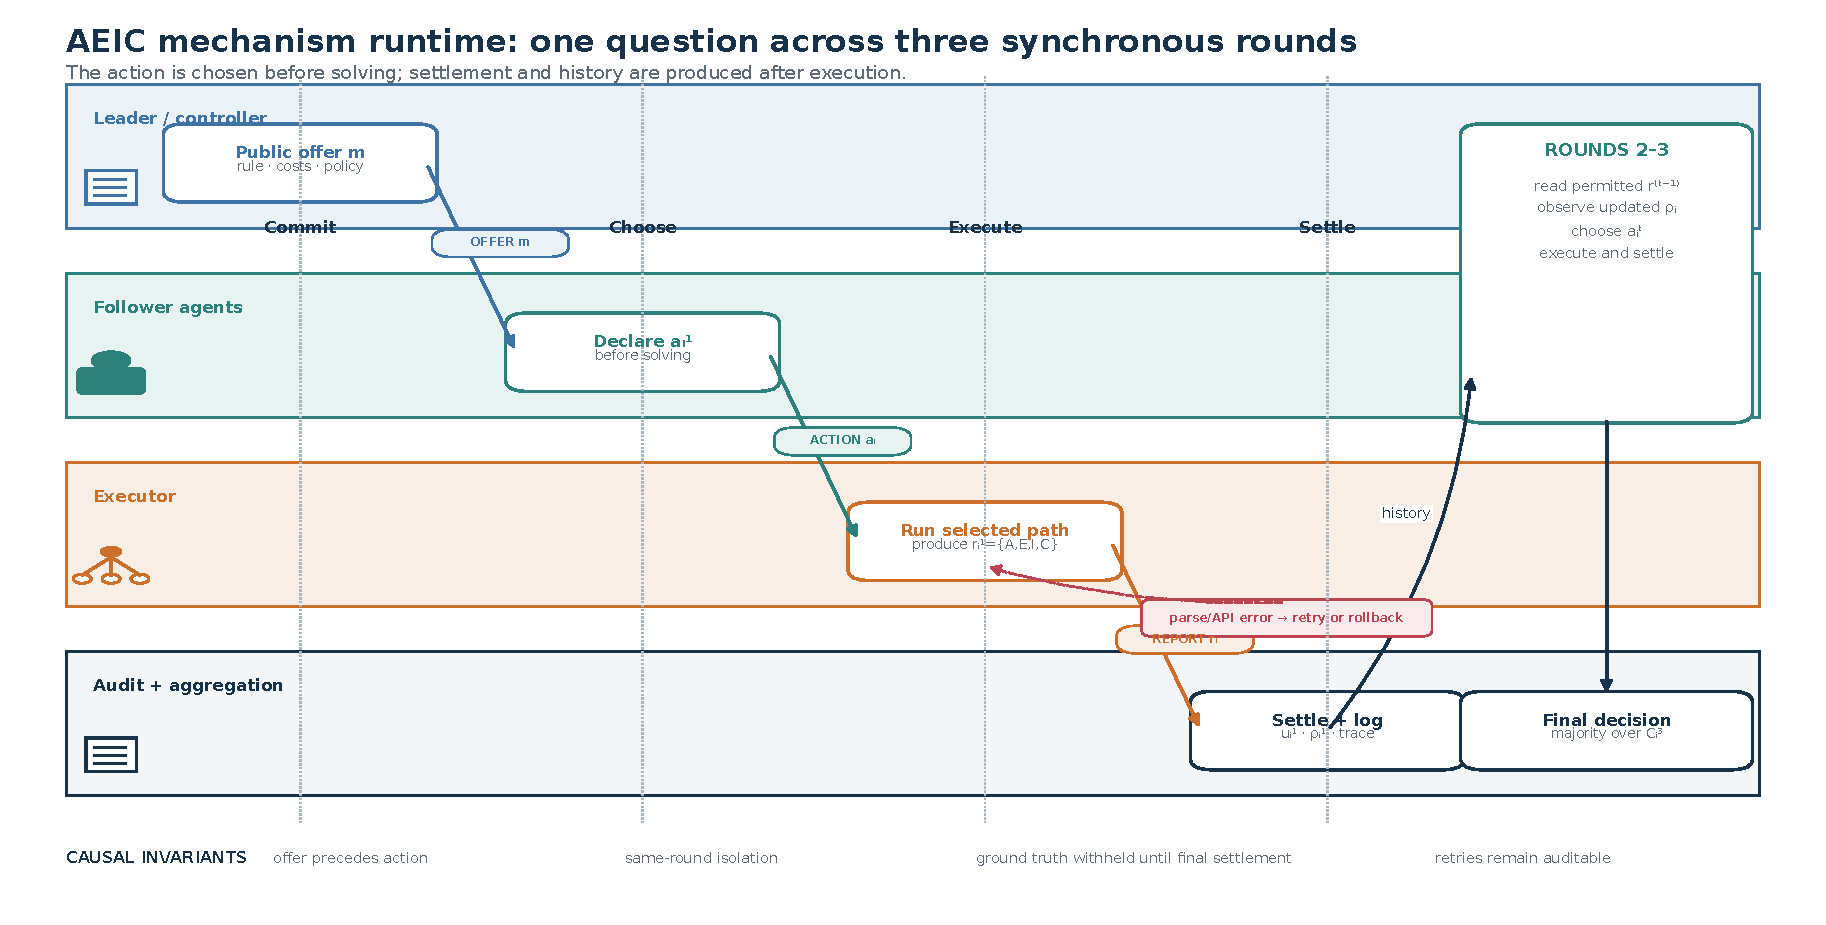
\includegraphics[width=\textwidth]{../figures/fig2_runtime_sequence.pdf}
\caption{Runtime sequence for one question. The four horizontal lanes separate controller commitment, follower choice, enforced execution, and settlement. Cross-round history is generated only after the current round has been logged, preserving same-round isolation.}
\label{fig:runtime}
\end{figure}

\paragraph{Choice before execution.}
Every agent first receives only the public contract, its visible reputation, the permitted information, and the question. It returns a single action. A second call executes the selected action. \textsc{Verify} adds a third audit-and-revision call. A formatting repair may be called only when JSON parsing fails; it is instructed to preserve the attempted conclusion and add no facts. All calls and token counts remain logged.

\paragraph{Pairing and aggregation.}
All mechanisms for a question share the question-level seed. The final panel decision is majority vote over explicit $C$ fields in the third round. High effort is defined before analysis as \textsc{AEIC} or \textsc{Verify}. Statistical tests operate at the natural paired unit: agent-round for the binary action and question for final correctness. We use exact McNemar tests for paired binary outcomes and paired rank tests for continuous outcomes, applying Holm correction within each registered contrast family.

\paragraph{Frozen provenance.}
Records use a versioned schema that requires the offer, chosen action, report, visible peers, reward, realized cost, reputation snapshots, raw response, action trace, latency, and token use before a record can be marked complete. Each suite passes an expected-versus-present matrix check, is frozen with SHA-256 provenance, and is independently recomputed from canonical question-level JSONL. The final manifest contains eight complete suites and 5,850 question-level records; no suite has missing, incomplete, unexpected, route-invalid, or schema-invalid records.
